%GLOSSARYA
%%%%%%%%%%%%%%%%%%%%%%%%%%%
%%%% Put the following at the top of each .tex file  %
\pagestyle{fancy}
\setcounter{page}{1}
\rhead{Glossary Part A}
\lhead{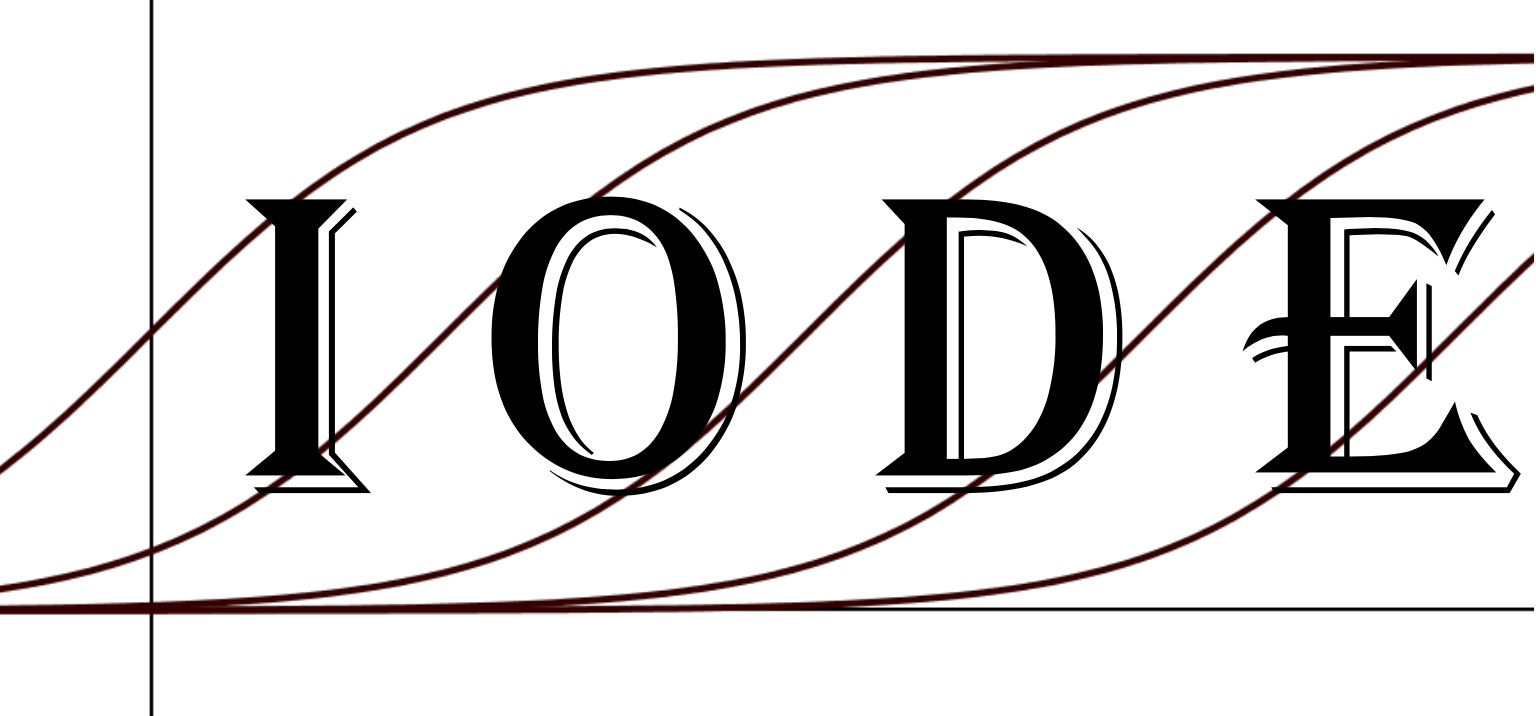
\includegraphics[width=1.25cm]{IODE-logo.png}}
\rfoot{Glossary Part A Page \thepage}
\lfoot{}
\cfoot{}
\fancypagestyle{firstfooter}{\footskip = 50pt}
\renewcommand{\footrulewidth}{.4pt}
%%%%%%%%%%%%%%%%%%%%%%%%%%%
\vspace*{-20pt} \thispagestyle{firstfooter}
\pagebegin{Glossary for First Order Differential Equations}
\begin{description}
\item[Analytic approach:] In this course, use have two analytic approaches \textbf{separation of variables} and the technique for \textbf{first order linear differential equations}. These approaches provide either general or particular solutions in algebraic or analytic form.
\item[Autonomous derivative graph:] A graph of $\frac{dy}{dt}$ vs. $y$, when $\frac{dy}{dt}$ is an autonomous differential equation.
\item[Autonomous differential equation:] A differential equation where the derivative is dependent only on the dependent variable. For example $\frac{dy}{dt}=2y-3$ is autonomous, but $\frac{dy}{dt} = 2t -3$ is not autonomous. 
\item[Bifurcation diagram:] A plot of equilibrium solutions versus a parameter. Additionally, one can show phase lines on the graph which show whether equilibrium solutions are stable (attractor), unstable (repeller), or semi-stable (node).
\item[Bifurcation value:] A value of the parameter for which there is a change in the number or type of equilibrium solutions.
\item[Differential equation:] A differential equation is also known as a \textbf{rate of change equation}. An equation for an unknown function in terms of its derivative. Suppose $y = y(t)$ is some unknown function, then a differential equation, or rate of change equation, would express the rate of change, $\frac{dy}{dt}$, in terms of $y$ and/or $t$. \textbf{First order} differential equation contains only the first derivative. \textbf{Second order} differential equations contains derivatives up to the second derivative. An \textbf{ordinary differential equation (ODE)} is a differential equation whose derivatives pertain to only one variable, typically derivatives with respect to time. A \textbf{partial differential equation (PDE)} is a differential equation whose derivatives pertain to multiple variables.
\item[Equilibrium solution:] A constant function that satisfies a given differential equation. There are three types of equilibrium solutions for first order differential equations: attractors (stable), repellers (unstable), and nodes (semi-stable). 
\item[Euler's method:] Informally referred to as the ``tip to tail" method; this is a numerical method to find approximate solutions to a given differential equation.
\item[First order linear differential equation:] A differential equation that can be written in the form $\frac{dy}{dt}+ g(t)y =r(t)$, where $g(t)$ and $r(t)$ are both continuous functions. This type of differential equation is solved using the analytic technique of \textbf{reverse product rule.}
\item[Initial condition or initial value:] A specific point through which the solution to a differential equation will pass. Usually expressed as $y_{t_0} = y_0$. For example, $y(0)=2$ (or $y(2)=6$) could be an initial condition that is then used to determine the \textbf{particular solution} from the \textbf{general solution}.
\item[Initial value problem (IVP):] A differential equation together with an initial condition (initial value) is called an Initial Value Problem (IVP).
\item[Integrating factor:] See \textbf{reverse product rule}.
\item[Numerical approach:] Provides numerical approximations to an initial value problem. One such method is \textbf{Euler's method}. Other methods include the Improved Euler's method and the \textbf{Runge-Kutta} method.
\item[Qualitative / graphical approach] An approach to solving a differential equation that considers slopes and how the solution follows the slopes in a field.
\item[Reverse product rule:] A technique for solving a \textbf{first order linear differential equation} by introducing an unknown function $u$ to help ``undo'' the product rule. $u$ is sometimes called an \textbf{integrating factor}.
\item[Runge-Kutta (RK4) method:] A fourth order method used in solving differential equations numerically. Contrast with \textbf{Euler's method} which is first order.
\item[Separable differential equation:] Differential equation that can be written in the form $\frac{dy}{dx}=f(y)g(x)$ and, when possible, solved using the analytic technique of \textbf{separation of variables}.
\item[Separation of variables:] An analytic technique to solve a differential equation of the form $\frac{dy}{dx}=f(y)g(x)$ by separating the variables (i.e., by rewriting it as $\frac{dy}{f(y)}=g(x)dx$) and integrating both sides if possible.
\item[Slope field:] A graphical representation of the slopes at many different points in a coordinate plane where each slope is determined by the derivative (rate of change) at any point in the plane. Slope fields can be used to sketch in graphs of solution functions. A curve that follows the slopes is the graphical analogue of inserting a function into the differential equation with the result giving a true statement.
\item[Solution to a differential equation:] Solutions to a rate of change equation are functions that satisfy the rate of change equation.
\begin{description}
\item[Exact solution:] A function that satisfies a given differential equation. That is, when the function is inserted into the differential equation a true statement results.
\item[Explicit solution:] The general solution has been written so that it is in the form $y(t) = e^{2t}$. Contrast this with \textbf{implicit solution}.
\item[General solution:] An algebraic (sometimes referred to as analytic) representation of the family of functions that solve a given differential equation.
\item[Implicit solution:] The general solution has been left in a form that has not been (or cannot be) algebraically solved. For example, $y(t)^5 + y(t) = e^{2t}$.
\item[Particular solution:] An algebraic (or analytic) representation of a specific function that solves the differential equation and contains a specified point, usually called the \textbf{initial value}. A differential equation together with an initial condition is referred to as an \textbf{initial value problem}.
\end{description}
\item[Uniqueness theorem:] Informally, the terms ``unique" or ``uniqueness" refers to whether or not two solution functions ever touch or cross each other. Refer to page 5.4 of the materials for the formal theorem.

\end{description}
